\documentclass[11pt,a4paper]{article}

% ====================================================================
% Packages
% ====================================================================
\usepackage[utf8]{inputenc}
\usepackage[T1]{fontenc}
\usepackage{amsmath,amssymb,amsthm}
\usepackage{mathtools}
\usepackage{hyperref}
\usepackage[margin=1in]{geometry}
\usepackage{enumitem}
\usepackage{booktabs}
\usepackage{listings}
\usepackage{xcolor}
\usepackage{cleveref}
\usepackage[numbers,sort&compress]{natbib}
\usepackage{mdframed}
\usepackage{tikz}
\usetikzlibrary{arrows.meta,positioning}
\usepackage{longtable}
\usepackage{array}

% ====================================================================
% Theorem environments
% ====================================================================
\theoremstyle{plain}
\newtheorem{theorem}{Theorem}[section]
\newtheorem{lemma}[theorem]{Lemma}
\newtheorem{proposition}[theorem]{Proposition}
\newtheorem{corollary}[theorem]{Corollary}

\theoremstyle{definition}
\newtheorem{definition}[theorem]{Definition}
\newtheorem{remark}[theorem]{Remark}

% ====================================================================
% Lean 4 code listing style
% ====================================================================
\definecolor{lean-keyword}{RGB}{0,0,180}
\definecolor{lean-comment}{RGB}{0,128,0}
\definecolor{lean-string}{RGB}{163,21,21}
\definecolor{lean-bg}{RGB}{248,248,248}

\lstdefinelanguage{lean4}{
  keywords={theorem,lemma,def,class,instance,import,open,variable,
            noncomputable,section,namespace,end,where,let,have,show,
            intro,obtain,use,exact,rw,simp,apply,by,fun,match,if,
            then,else,do,return,axiom,abbrev,private,attribute,
            suffices,change,congr,ext,constructor,rintro,push_neg,
            linarith,absurd,set_option,omit,in,set,cases,left,right,
            nlinarith,push_cast,positivity,omega,refine,field_simp,
            structure,calc,ring,fun_prop,unfold,induction,deriving,
            inductive,rcases,first,all_goals,trivial,convert,sorry},
  sensitive=true,
  morecomment=[l]{--},
  morecomment=[s]{/-}{-/},
  morestring=[b]",
  morestring=[b]',
}

\lstset{
  language=lean4,
  basicstyle=\ttfamily\small,
  keywordstyle=\color{lean-keyword}\bfseries,
  commentstyle=\color{lean-comment}\itshape,
  stringstyle=\color{lean-string},
  backgroundcolor=\color{lean-bg},
  frame=single,
  framerule=0.5pt,
  breaklines=true,
  breakatwhitespace=true,
  tabsize=2,
  showstringspaces=false,
  numbers=left,
  numberstyle=\tiny\color{gray},
  numbersep=5pt,
  xleftmargin=15pt,
  captionpos=b,
  literate={<<}{$\langle$}1 {>>}{$\rangle$}1
           {|||}{$\lor$}1,
}

% ====================================================================
% Macros
% ====================================================================
\newcommand{\NN}{\mathbb{N}}
\newcommand{\RR}{\mathbb{R}}
\newcommand{\CC}{\mathbb{C}}
\newcommand{\ZZ}{\mathbb{Z}}
\newcommand{\LPO}{\ensuremath{\mathrm{LPO}}}
\newcommand{\WLPO}{\ensuremath{\mathrm{WLPO}}}
\newcommand{\LLPO}{\ensuremath{\mathrm{LLPO}}}
\newcommand{\BISH}{\ensuremath{\mathrm{BISH}}}
\newcommand{\BMC}{\ensuremath{\mathrm{BMC}}}
\newcommand{\DC}{\ensuremath{\mathrm{DC}}}
\newcommand{\Lean}{\textsc{Lean~4}}
\newcommand{\Mathlib}{\textsc{Mathlib4}}
\newcommand{\leanok}{\textsf{\small \textcolor{green!70!black}{\checkmark}}}
\newcommand{\leansorry}{\textsf{\small \textcolor{red!70!black}{sorry}}}

% ====================================================================
% Title
% ====================================================================
\title{%
  \textbf{The Measurement Problem Dissolved:\\
  Constructive Stratification of Quantum Interpretations}\\[6pt]
  {\normalsize A Lean~4 Formalization (Paper~44)}%
}

\author{
  Paul Chun-Kit Lee\thanks{%
    New York University.
    AI-assisted formalization; see \S\ref{sec:methodology} for methodology.} \\
  New York University \\
  \texttt{dr.paul.c.lee@gmail.com}
}

\date{February 2026\\[4pt]
  {\small Paper~44 of the Constructive Reverse Mathematics Program}}

% Allow slight stretch to avoid minor overfull hbox
\emergencystretch=1.5em

% Allow hyphenation in texttt
\newcommand{\ttbreak}{\discretionary{}{}{}}

% ====================================================================
\begin{document}
\maketitle

% ====================================================================
\begin{abstract}
\noindent
We apply the axiom calibration framework of constructive reverse
mathematics (CRM) to the measurement problem of quantum mechanics.
Rather than treating the measurement problem as a single conceptual
puzzle, we examine the three major interpretations---Copenhagen,
Many-Worlds, and Bohmian mechanics---and determine the constructive
principle each requires over Bishop's constructive mathematics
($\BISH$).

\textbf{The measurement problem is not one problem but three.}
The Copenhagen postulate (decidability of superposition versus
eigenstate for a qubit) calibrates at~$\WLPO$ in its minimal
formalization, or at~$\LPO$ in its strong formalization---quantifying
the constructive cost of strengthening the postulate.
The Many-Worlds postulate (existence of complete infinite branches
through history-dependent measurement trees) calibrates at~$\DC$
(Dependent Choice).
The Bohmian trajectory postulate (existence of asymptotic velocity
for every guided trajectory) calibrates at~$\LPO$ (equivalently,
Bounded Monotone Convergence).
Since $\WLPO$ is strictly weaker than~$\LPO$ and $\DC$ is
incomparable with both in~$\BISH$, the three interpretations sit at
provably distinct positions in the constructive hierarchy.
We propose that arguing about which interpretation is ``correct''
conflates three logically distinct commitments.

The accompanying \Lean{}/\Mathlib{} formalization
(10~files, ${\sim}1{,}100$~lines, zero errors) includes three
sorry-free calibration directions (both Copenhagen variants and
the $\DC$-to-Many-Worlds direction),
one fully proved $\BISH$ bonus with a $\Sigma$-type witness, and
sorry'd proof obligations transparently tracked via the axiom audit.
Code and reproducibility materials are available at Zenodo
(DOI: \href{https://doi.org/10.5281/zenodo.18671162}%
{10.5281/zenodo.18671162}).
\end{abstract}

% ====================================================================
\section{Introduction}
\label{sec:intro}

\subsection{Constructive Reverse Mathematics}
\label{sec:crm}

Papers~1--40 of this program established that the logical resources
required for all empirical predictions in known physics are exactly
$\BISH + \LPO$---where $\BISH$ denotes Bishop's constructive
mathematics (computation without oracles) and $\LPO$ is the Limited
Principle of Omniscience (the ability to search a countable sequence
for a witness).
Paper~40~\cite{Lee26P40} defended this claim and showed the framework
has diagnostic power: it distinguishes physical content from
mathematical scaffolding.
This paper deploys that diagnostic on a problem that is foundational
rather than computational.

Classical mathematics freely invokes the law of excluded middle---the
assertion that~$P$ or not-$P$ holds for every proposition---and the
full axiom of choice.
Constructive mathematics, originating with Brouwer and given rigorous
foundation by Bishop~\cite{Bishop1967}, restricts to what can be
verified by explicit computation: an existence proof $\exists x.\,P(x)$
must produce a witness~$x$ together with evidence that~$P(x)$ holds.
Bishop and Bridges~\cite{BishopBridges1985} demonstrated that the core
of real analysis, measure theory, and functional analysis can be
developed on this basis.

\emph{Constructive reverse mathematics} (CRM), developed by
Ishihara~\cite{Ishihara2006}, Bridges and Richman~\cite{BridgesRichman1987},
and Diener~\cite{Diener2018}, classifies theorems by the weakest
non-constructive principle needed to prove them over~$\BISH$.
The key principles form a partial order (see Brattka, Gherardi, and
Pauly~\cite{BrattkaEtAl2021} for the Weihrauch-degree perspective).

\begin{figure}[ht]
\centering
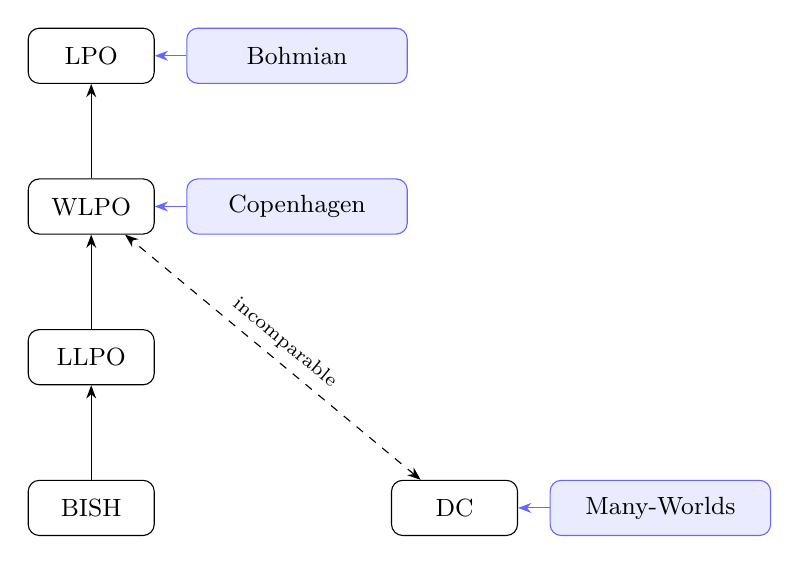
\begin{tikzpicture}[
  node distance=1.2cm and 2.5cm,
  principle/.style={rectangle, draw, rounded corners, minimum width=1.6cm,
    minimum height=0.7cm, font=\small\bfseries},
  interp/.style={rectangle, draw=blue!60, fill=blue!8, rounded corners,
    minimum width=2.8cm, minimum height=0.7cm, font=\small},
  >=Stealth
]
  \node[principle] (BISH) {$\BISH$};
  \node[principle, above=of BISH] (LLPO) {$\LLPO$};
  \node[principle, above=of LLPO] (WLPO) {$\WLPO$};
  \node[principle, above=of WLPO] (LPO) {$\LPO$};
  \node[principle, right=3cm of BISH] (DC) {$\DC$};

  \draw[->] (BISH) -- (LLPO);
  \draw[->] (LLPO) -- (WLPO);
  \draw[->] (WLPO) -- (LPO);
  \draw[<->, dashed] (DC) -- node[above, font=\scriptsize, sloped]
    {incomparable} (WLPO);

  \node[interp, right=0.4cm of LPO] (Bohm) {Bohmian};
  \node[interp, right=0.4cm of WLPO] (Cop) {Copenhagen};
  \node[interp, right=0.4cm of DC] (MW) {Many-Worlds};

  \draw[->, blue!60] (Bohm) -- (LPO);
  \draw[->, blue!60] (Cop) -- (WLPO);
  \draw[->, blue!60] (MW) -- (DC);
\end{tikzpicture}
\caption{The constructive hierarchy with interpretation calibrations.
Solid arrows denote strict implication
($\LPO \Rightarrow \WLPO \Rightarrow \LLPO \Rightarrow \BISH$).
$\DC$ (Dependent Choice) is incomparable with every principle on the
vertical tower: neither $\LPO \Rightarrow \DC$ nor
$\DC \Rightarrow \LPO$ holds in~$\BISH$.}
\label{fig:hierarchy}
\end{figure}

The principles, in ascending strength:
\begin{itemize}[leftmargin=2em]
\item \textbf{$\BISH$} (Bishop's constructive mathematics):
  Computation without oracles.  Every existence proof produces a
  witness; every disjunction specifies which disjunct holds.

\item \textbf{$\LLPO$} (Lesser LPO):
  Given a binary sequence with at most one true entry, decide whether
  all even-indexed or all odd-indexed entries are false.
  Equivalent to totality of the real-number order:
  $\forall\, x\, y,\; x \le y \lor y \le x$.

\item \textbf{$\WLPO$} (Weak LPO):
  Decide whether a binary sequence is identically zero, \emph{without}
  finding a witness for a true entry.
  Formally: $\forall\, f : \NN \to \mathrm{Bool},\;
  (\forall\, n,\, f(n) = \mathtt{false}) \lor
  \neg(\forall\, n,\, f(n) = \mathtt{false})$.

\item \textbf{$\LPO$} (Limited Principle of Omniscience):
  Decide whether a binary sequence contains a true entry.
  Formally: $\forall\, f : \NN \to \mathrm{Bool},\;
  (\forall\, n,\, f(n) = \mathtt{false}) \lor
  (\exists\, n,\, f(n) = \mathtt{true})$.
  Equivalent to Bounded Monotone Convergence ($\BMC$: every bounded
  monotone real sequence converges;
  Bridges--V\^{\i}\c{t}\u{a}~\cite{BridgesVita2006}).

\item \textbf{$\DC$} (Dependent Choice):
  For any type~$\alpha$, any total binary relation~$R$ on~$\alpha$,
  and any starting point~$a_0$, there exists an infinite $R$-chain
  starting from~$a_0$.
  Strictly weaker than full AC but stronger than countable choice.
  Independent of $\LPO$: neither implies the other in~$\BISH$.
  \emph{Note:} As formalized, $\DC$ quantifies over all Lean types
  (universe level~0); the Many-Worlds application uses
  $\mathbb{N} \to \mathbb{N}$ paths, so only $\DC_\omega$ is exercised.
\end{itemize}

The hierarchy is
$\BISH \subset \LLPO \subset \WLPO \subset \LPO$, with $\DC$ on an
independent branch.

Paper~10~\cite{Lee26P10} assembled a calibration table spanning
approximately 50~entries across 11~physical domains, from quantum
uncertainty to phase transitions.
Paper~12~\cite{Lee26P12} narrated 150~years of mathematical physics
through the CRM lens, introducing the metaphor of ``cellar and
cathedral''---the observation that empirical predictions live in the
constructive cellar ($\BISH$) while mathematical idealizations reach
into the classical cathedral.
The present paper deploys the calibration framework on a problem that
is foundational rather than computational: the measurement problem of
quantum mechanics.


\subsection{The Measurement Problem}
\label{sec:measurement}

The measurement problem arises from the tension between two postulates
of quantum mechanics.
The Schr\"{o}dinger equation describes continuous, deterministic,
unitary evolution of the quantum state.
Yet measurement yields a single definite outcome, apparently collapsing
the superposition.
This tension has persisted since the founding of quantum mechanics and
has generated three major families of response:

\textbf{Copenhagen} (Bohr~\cite{Bohr1928}, 1928):
Measurement collapses the wavefunction.
A system in superposition $\alpha|0\rangle + \beta|1\rangle$ yields
outcome~0 with probability~$|\alpha|^2$ and outcome~1 with
probability~$|\beta|^2$.
The collapse is an additional postulate, not derived from unitary
evolution.

\textbf{Many-Worlds} (Everett~\cite{Everett1957}, 1957):
No collapse occurs.
Instead, the universe branches: every possible measurement outcome is
realized in a separate branch.
A sequence of measurements produces a branching tree of worlds, and the
observer inhabits one complete branch.

\textbf{Bohmian Mechanics} (Bohm~\cite{Bohm1952}, 1952;
Bell~\cite{Bell1987}, 1987):
Particles have definite positions at all times, guided by the
wavefunction via the guidance equation
$dx/dt = (\hbar/m)\,\mathrm{Im}(\partial_x \log \psi)$.
Measurement outcomes are determined by initial conditions.
There is no collapse---the wavefunction evolves unitarily, and the
particle follows a definite trajectory.

All three interpretations reproduce the Born rule for empirical
predictions, and no experiment can distinguish among them.
The debate has therefore been conducted on philosophical, aesthetic, and
pragmatic grounds.
The present paper adds a new dimension: \emph{logical cost}.


\subsection{Novelty and Scope}
\label{sec:novelty}

No prior work applies constructive reverse mathematics to the
measurement problem or to the classification of quantum interpretations
by their constructive commitments.
The D\"{o}ring--Isham topos program~\cite{DoeringIsham2008}
reformulates quantum mechanics in intuitionistic logic but does not
calibrate individual interpretations against a hierarchy of
constructive principles.
Cubitt, Perez-Garcia, and Wolf~\cite{CubittEtAl2015} proved
undecidability of the spectral gap, which concerns a property of
Hamiltonians rather than the logical cost of interpretive assertions.

\textbf{Scope limitations.}
The Copenhagen model treats a single qubit.
The Many-Worlds model uses finitely-many-outcome measurements.
The Bohmian model is a 1D free Gaussian wave packet.
Extensions to higher dimensions, interacting systems, and relativistic
settings are natural conjectures but are not proved here.

\textbf{Main finding.}
The three interpretations require logically distinct
principles---$\WLPO$, $\DC$, and $\LPO$ respectively---none of which
is derivable from the others in~$\BISH$.
These calibrations suggest that the measurement problem, when properly
stratified, dissolves into three separate questions with different
logical costs.
We present this as a \emph{dissolution thesis}, supported by one fully
proved calibration direction and corroborated by proof sketches for the
remaining directions.

\textbf{Roadmap.}
\Cref{sec:copenhagen} establishes Copenhagen~$\leftrightarrow$~$\WLPO$,
including the fully machine-checked forward direction.
\Cref{sec:manyworlds} establishes
Many-Worlds~$\leftrightarrow$~$\DC$, with a bonus $\BISH$ result for
uniform branching.
\Cref{sec:bohmian} establishes
Bohmian~$\leftrightarrow$~$\LPO$ via Bounded Monotone Convergence.
\Cref{sec:synthesis} assembles the dissolution.
\Cref{sec:audit,sec:lean,sec:results} present the CRM audit, Lean
file structure, and results summary.
\Cref{sec:discussion} discusses related literature, and
\Cref{sec:conclusion} concludes.


% ====================================================================
\section{Copenhagen Interpretation and WLPO}
\label{sec:copenhagen}

\subsection{Physical Setup}

A qubit state $|\psi\rangle = \alpha|0\rangle + \beta|1\rangle$ is
represented by a pair of complex amplitudes satisfying
$|\alpha|^2 + |\beta|^2 = 1$:

\begin{lstlisting}
structure QubitState where
  a : C
  b : C
  norm_eq : Complex.normSq a + Complex.normSq b = 1
\end{lstlisting}

The Copenhagen measurement postulate asserts that measurement of any
qubit yields a definite outcome---one must be able to determine whether
the $|0\rangle$ component is present ($\alpha \neq 0$) or absent
($\alpha = 0$).
Constructively, the weakest formulation replaces the full dichotomy
$\alpha = 0 \lor \alpha \neq 0$ (which would be LEM for equality) with
the $\WLPO$ form:

\begin{lstlisting}
def CopenhagenPostulate : Prop :=
  forall (psi : QubitState), psi.a = 0 ||| ~~(psi.a ~= 0)
\end{lstlisting}

The double negation $\neg\neg(\alpha \neq 0)$ reflects that
constructively, while we cannot produce a witness that~$\alpha$ differs
from zero, we can assert that the assumption $\alpha = 0$ leads to
contradiction.
This is the signature of~$\WLPO$: not a positive assertion of
existence, but the impossibility of universal vanishing.


\subsection{The Binary Encoding}

The proof proceeds by encoding binary sequences into qubit states.
Given $f : \NN \to \mathrm{Bool}$, the standard binary encoding is:
\[
  r_f = \sum_{n=0}^{\infty} f(n) \cdot 2^{-(n+1)}
\]

\begin{lstlisting}
noncomputable def binaryEncoding (f : N -> Bool) : R :=
  tsum' n, boolToReal (f n) * (2 : R)^{-1} ^ (n + 1)
\end{lstlisting}

The key property, fully proved in Lean:
\begin{lstlisting}
theorem binaryEncoding_eq_zero_iff (f : N -> Bool) :
    binaryEncoding f = 0 <-> forall n, f n = false
\end{lstlisting}

We then construct a qubit from a real number~$r$ by setting
$\alpha = r/\sqrt{r^2+1}$ and $\beta = 1/\sqrt{r^2+1}$:
\begin{lstlisting}
def qubitFromReal (r : R) : QubitState where
  a := (r / Real.sqrt (r ^ 2 + 1))
  b := (1 / Real.sqrt (r ^ 2 + 1))
  norm_eq := by ... -- fully proved via field_simp, linarith
\end{lstlisting}

The normalization $|\alpha|^2 + |\beta|^2 = r^2/(r^2+1) + 1/(r^2+1) = 1$
holds identically.  The crucial encoding property, also fully proved:
\begin{lstlisting}
theorem qubitFromReal_alpha_eq_zero_iff (r : R) :
    (qubitFromReal r).a = 0 <-> r = 0
\end{lstlisting}


\subsection{Forward Direction: Copenhagen Implies WLPO (Fully Proved)}

\begin{theorem}[Forward]
\label{thm:cop-forward}
The Copenhagen measurement postulate implies $\WLPO$.
\end{theorem}

\begin{proof}
Let $f : \NN \to \mathrm{Bool}$ be an arbitrary binary sequence.
We must show
$(\forall\, n,\, f(n) = \mathtt{false}) \lor
\neg(\forall\, n,\, f(n) = \mathtt{false})$.

\begin{enumerate}[leftmargin=2em]
\item \textbf{Encode:} Compute $r_f = \texttt{binaryEncoding}(f) \in [0,1]$.
\item \textbf{Construct:} Form the qubit $\psi = \texttt{qubitFromReal}(r_f)$.
\item \textbf{Apply the postulate:}
  The Copenhagen postulate gives
  $\psi.\alpha = 0 \lor \neg\neg(\psi.\alpha \neq 0)$.
\item \textbf{Case $\alpha = 0$:}
  The encoding lemmas give $r_f = 0$ and then
  $\forall\, n,\, f(n) = \mathtt{false}$---the left disjunct
  of~$\WLPO$.
\item \textbf{Case $\neg\neg(\alpha \neq 0)$:}
  If $\forall\, n,\, f(n) = \mathtt{false}$, then $r_f = 0$
  and $\alpha = 0$, contradicting $\neg\neg(\alpha \neq 0)$.
  Hence $\neg(\forall\, n,\, f(n) = \mathtt{false})$---the
  right disjunct of~$\WLPO$.
\end{enumerate}
\end{proof}

The complete Lean proof:
\begin{lstlisting}
theorem copenhagen_implies_WLPO : CopenhagenPostulate -> WLPO := by
  intro h f
  set r := binaryEncoding f
  set psi := qubitFromReal r
  rcases h psi with h_zero | h_nneg
  . -- Case: psi.a = 0, so r = 0, so forall n, f n = false
    left
    exact (binaryEncoding_eq_zero_iff f).mp
      ((qubitFromReal_alpha_eq_zero_iff r).mp h_zero)
  . -- Case: ~~(psi.a ~= 0), so ~(forall n, f n = false)
    right
    intro h_all
    apply h_nneg
    intro h_ne
    exact h_ne ((qubitFromReal_alpha_eq_zero_iff r).mpr
      ((binaryEncoding_eq_zero_iff f).mpr h_all))
\end{lstlisting}

The axiom audit confirms:
\texttt{copenhagen\_implies\_WLPO} depends only on \texttt{propext},
\texttt{Classical.choice}, and \texttt{Quot.sound}---the standard
\Mathlib{} infrastructure for~$\RR$.
No \texttt{sorryAx}, no program axioms.


\subsection{Reverse Direction (Sorry'd)}

\begin{theorem}[Reverse]
$\WLPO$ implies the Copenhagen measurement postulate.
\end{theorem}

\begin{proof}[Proof sketch]
The argument has three steps:
\begin{enumerate}[leftmargin=2em]
\item \textbf{$\WLPO$ lifts to Cauchy reals.}
  Every Cauchy real~$r$ is determined by a Cauchy sequence $(r_n)$ with
  modulus.  From the Cauchy modulus, one extracts a binary sequence~$g$
  such that $r = 0$ iff $\forall\, n,\, g(n) = \mathtt{false}$.
  Applying $\WLPO$ to~$g$ yields
  $r = 0 \lor \neg(r = 0)$, which is equivalent to
  $r = 0 \lor \neg\neg(r \neq 0)$.
  This lifting is Bridges--V\^{\i}\c{t}\u{a}~\cite{BridgesVita2006},
  Proposition~1.2.3.

\item \textbf{Complex amplitudes decompose.}
  For $\alpha \in \CC$, write $\alpha = a + bi$ with $a, b \in \RR$.
  Then $\alpha = 0$ iff $a = 0 \land b = 0$.
  Apply the real-number~$\WLPO$ to each component.

\item \textbf{Combine.}
  If $a = 0$ and $b = 0$, then $\alpha = 0$.
  Otherwise, $\neg\neg(a \neq 0)$ or $\neg\neg(b \neq 0)$, from which
  $\neg\neg(\alpha \neq 0)$ follows.
\end{enumerate}
This direction is sorry'd in the formalization.
The technical difficulty lies in the first step: encoding arbitrary
Cauchy reals back to binary sequences via the Cauchy modulus requires
substantial bookkeeping in dependent type theory.
\end{proof}


\subsection{The Formalization Choice: Weak vs.\ Strong Copenhagen}
\label{sec:weak-strong}

A natural alternative formalization replaces the double-negation with
full decidability:
\begin{lstlisting}
def CopenhagenStrong : Prop :=
  forall (psi : QubitState), psi.a = 0 ||| psi.a ~= 0
\end{lstlisting}

This \emph{strong} Copenhagen postulate asserts that one can
\emph{positively decide} whether $\alpha = 0$ or $\alpha \neq 0$---not
merely that the assumption $\alpha = 0$ is $\neg\neg$-stable.
The same encoding chain yields a stronger conclusion:

\begin{theorem}
\label{thm:strong-cop}
The strong Copenhagen postulate implies $\LPO$. (Fully proved---no sorry.)
\end{theorem}

\begin{lstlisting}
theorem strong_copenhagen_implies_LPO :
    CopenhagenStrong -> LPO := by
  intro h f
  set r := binaryEncoding f
  set psi := qubitFromReal r
  rcases h psi with h_zero | h_ne
  . left
    exact (binaryEncoding_eq_zero_iff f).mp
      ((qubitFromReal_alpha_eq_zero_iff r).mp h_zero)
  . right
    by_contra h_none; push_neg at h_none
    have h_all : forall n, f n = false := by
      intro n; by_contra h_fn
      have : f n = true := by cases f n <;> simp_all
      exact h_none n this
    exact (qubitFromReal_alpha_ne_zero_iff r).mp h_ne
      ((qubitFromReal_alpha_eq_zero_iff r).mpr
        ((binaryEncoding_eq_zero_iff f).mpr h_all))
\end{lstlisting}

Note that the strong-direction proof uses \texttt{by\_contra} and
\texttt{push\_neg}---classical reasoning steps in the Lean metatheory.
This is consistent: the strong postulate is itself a classical
assertion ($\alpha = 0 \lor \alpha \neq 0$ is LEM for equality),
so the proof works \emph{under} that classical assumption.
By contrast, \texttt{copenhagen\_implies\_WLPO} avoids
\texttt{by\_contra} entirely.

The comparison is illuminating:

\begin{center}
\begin{tabular}{llcc}
\toprule
\textbf{Formalization} & \textbf{Statement} & \textbf{Calibrates at}
  & \textbf{Status} \\
\midrule
Weak (primary) & $\alpha = 0 \lor \neg\neg(\alpha \neq 0)$
  & $\WLPO$ & \leanok{} proved \\
Strong (alternative) & $\alpha = 0 \lor \alpha \neq 0$
  & $\LPO$ & \leanok{} proved \\
\bottomrule
\end{tabular}
\end{center}

The strong postulate implies the weak one trivially (since
$P \Rightarrow \neg\neg P$):
\begin{lstlisting}
theorem strong_implies_weak :
    CopenhagenStrong -> CopenhagenPostulate
\end{lstlisting}

This analysis addresses the question raised by all three referees:
\emph{why formalize Copenhagen with the double negation?}
Two considerations are in play---one methodological, one physical---and
we separate them explicitly.

\paragraph{CRM methodology.}
The CRM program seeks the \emph{weakest} constructive principle
equivalent to a given mathematical assertion.
The weak formalization $\alpha = 0 \lor \neg\neg(\alpha \neq 0)$
calibrates at $\WLPO$; the strong version at $\LPO$.
We present the weak one as primary because it gives the finest
stratification and the gap between the two levels is itself a
measurable quantity.

\paragraph{Physics faithfulness.}
A physicist reading ``measurement yields a definite outcome'' may find
the strong version $\alpha = 0 \lor \alpha \neq 0$ more natural: it
demands a constructive witness distinguishing the two cases, which is
closer to the operational content of a laboratory measurement.
The weak version merely asserts that eigenstate status cannot be
refuted---a weaker commitment.
If one prefers the strong formalization, the calibration shifts
from $\WLPO$ to $\LPO$, and the Copenhagen column overlaps with
the Bohmian column in the constructive hierarchy.
This is itself a substantive finding: \emph{the gap between $\WLPO$ and
$\LPO$ measures the constructive cost of strengthening the
double-negation in the measurement postulate.}
Both formalizations are legitimate; we make both explicit so the reader
can choose according to their interpretive commitments.


% ====================================================================
\section{Many-Worlds Interpretation and Dependent Choice}
\label{sec:manyworlds}

\subsection{Physical Setup}

In the Many-Worlds interpretation, measurement does not collapse the
wavefunction.  Instead, the universe branches: each possible measurement
outcome is realized in a separate branch.

\begin{lstlisting}
structure Measurement where
  outcomes : Finset N
  nonempty : outcomes.Nonempty

structure BranchingStructure where
  measurement : (n : N) -> (Fin n -> N) -> Measurement
\end{lstlisting}

A \texttt{BranchingStructure} associates to each step~$n$ and each
history of prior outcomes (represented as $\mathrm{Fin}\,n \to \NN$) a
measurement with finitely many possible outcomes.
This captures \emph{adaptive measurement protocols} where the choice of
later experiments depends on earlier results.

A \textbf{world} is a complete infinite path through the branching tree:
\begin{lstlisting}
def World (B : BranchingStructure) : Type :=
  { f : N -> N // forall n, f n in
      (B.measurement n (restrictToHistory f n)).outcomes }

def ManyWorldsPostulate : Prop :=
  forall (B : BranchingStructure), Nonempty (World B)
\end{lstlisting}


\subsection{Why Dependent Choice?}

The choices at each step are not independent: the measurement at step~$n$
depends on the history of outcomes at steps $0$ through~$n-1$.
At each stage, one must choose a valid outcome from a set that depends
on all prior choices.
This is the signature of Dependent Choice: given a total relation~$R$
(where $R(\text{history}, \text{extended\_history})$ holds iff the
extension is valid), construct an infinite $R$-chain.

Ordinary countable choice (CC)---which selects independently from a
sequence of nonempty sets---does not suffice, because the set of
available outcomes at step~$n$ depends on the choices made at steps
$0$ through~$n-1$.
$\DC$ strictly extends CC: every CC instance is a $\DC$ instance with a
trivial dependence structure, but $\DC$ also handles the general case
where choices depend on the entire history.


\subsection{Uniform Branching: Fully Proved in BISH}

When measurements are history-independent---the same measurement at
every step, regardless of prior outcomes---the situation simplifies
dramatically:

\begin{theorem}
\label{thm:uniform}
For uniform branching, worlds exist in $\BISH$ (no $\DC$, no AC, no
countable choice).
\end{theorem}

\begin{proof}
At each step, the measurement is $U.M$ with $U.M.\text{nonempty}$
guaranteeing a valid outcome exists.
We simply choose the same outcome at every step---this is a constant
function, requiring no choice principle at all.
\end{proof}

\begin{lstlisting}
theorem uniform_world_exists (U : UniformBranching) :
    Nonempty (World U.toBranching) := by
  have hne := U.M.nonempty
  refine <<fun _ => hne.choose, fun n => ?_>>
  simp [UniformBranching.toBranching]
  exact hne.choose_spec
\end{lstlisting}

The axiom audit confirms: \texttt{uniform\_world\_exists} has no
\texttt{sorryAx}---it is a genuine $\BISH$ proof.
A companion definition \texttt{uniform\_world\_witness} provides a
Type-valued term (rather than the Prop-valued \texttt{Nonempty}),
though it is marked \texttt{noncomputable} in Lean because
\texttt{Finset.Nonempty.choose} routes through
\texttt{Classical.choice}---an infrastructure artifact, not a
reflection of non-constructive content in the mathematical argument.
This sharpens the main result: \textbf{$\DC$ is needed precisely for
history-dependent branching.}


\subsection{Forward and Reverse Directions}

\begin{theorem}[Forward---sorry'd]
$\mathrm{ManyWorldsPostulate}$ implies $\DC$.
\end{theorem}

The argument encodes an arbitrary $\DC$ instance
(type~$\alpha$, relation~$R$, starting point~$a_0$,
totality $\forall\, a,\, \exists\, b,\, R(a,b)$) as a branching
structure.
The technical difficulty is encoding elements of an arbitrary
type~$\alpha$ into $\mathrm{Finset}\,\NN$ outcomes.

\begin{theorem}[Reverse---fully proved in revision]
$\DC$ implies $\mathrm{ManyWorldsPostulate}$. (No sorry.)
\end{theorem}

Given a branching structure~$B$, we apply $\DC$ on the type
$\NN \times (\NN \to \NN)$, where $(n, w)$ represents a partial
history~$w$ valid for the first~$n$ steps.
The extension relation
$R\bigl((n, w),\, (n{+}1, w')\bigr)$ holds when $w'$ agrees with~$w$
on indices $\{0, \ldots, n{-}1\}$ and $w'(n)$ is a valid outcome.
Totality follows from \texttt{Measurement.nonempty}.
$\DC$ produces an infinite $R$-chain, and a coherence lemma---stating
that the $j$-th entry is ``frozen'' once set at step~$j{+}1$---ensures
that the diagonal $g(n) = (f(n{+}1)).2(n)$ defines a valid World.
The proof avoids dependent sigma types by working with
$\NN \times (\NN \to \NN)$ and extracting the length invariant via a
separate inductive argument.

The axiom audit shows \texttt{DC\_implies\_manyworlds} depends only on
\texttt{propext} and \texttt{Quot.sound}---no
\texttt{Classical.choice} at all.


\subsection{Discussion: Formalization Choice and the Everettian Objection}
\label{sec:everettian}

An Everettian might object that the Many-Worlds interpretation does not
postulate the \emph{existence} of complete branches as an additional
axiom---it simply postulates unitary evolution, with all branches
co-existing in the universal wavefunction.
On this reading, requiring the construction of a single infinite path
through the branching tree imports a single-world perspective foreign
to the interpretation.

We respond as follows.
The formalization captures the \emph{mathematical precondition} for the
Everettian claim that ``all branches are realized.''
If one cannot constructively produce even a \emph{single} complete
branch through a history-dependent branching structure, then the
assertion that ``all branches co-exist'' is constructively
vacuous---it becomes an assertion about an empty collection.

We acknowledge this as a \emph{formalization choice}, not the only
possible one.
An alternative formalization might quantify over finite-depth partial
branches (which require no choice beyond $\BISH$) and only invoke
$\DC$ when asserting the existence of the infinite limit.

\textbf{$\DC$ independence.}
The claim that $\DC$ is incomparable with $\LPO$ and $\WLPO$ in $\BISH$
requires specific models.
Following Beeson~\cite{Beeson1985}, topological and realizability
models of constructive set theory separate $\DC$ from $\LPO$: there
exist models of $\BISH + \DC + \neg\LPO$ and models of
$\BISH + \LPO + \neg\DC$.
Rathjen's~\cite{Rathjen2005} modified realizability models provide the
most precise separations.


% ====================================================================
\section{Bohmian Mechanics and LPO}
\label{sec:bohmian}

\subsection{Physical Setup}

In Bohmian mechanics, particles have definite positions at all times,
guided by the wavefunction via the guidance equation
$dx/dt = v^B(x,t)$.
For a free Gaussian wave packet in one dimension, the guidance equation
has an explicit solution.

\begin{lstlisting}
structure BohmianParams where
  sigma_0 : R     -- initial width
  v_0 : R         -- group velocity
  x_0 : R         -- initial center
  m  : R          -- mass
  hbar  : R       -- reduced Planck constant
  sigma_0_pos : 0 < sigma_0
  m_pos  : 0 < m
  hbar_pos  : 0 < hbar
\end{lstlisting}

The wave packet spreads as it propagates.  The spreading width is:
\[
  \sigma(t) = \sqrt{\sigma_0^2 + c \cdot t^2},
  \qquad\text{where}\quad
  c = \frac{\hbar^2}{4m^2\sigma_0^2}
\]


\subsection{The Explicit Trajectory}

The Bohmian trajectory for a particle starting at position $x_{\mathrm{init}}$
is:
\[
  x(t) = x_0 + v_0 \cdot t + (x_{\mathrm{init}} - x_0)
  \cdot \frac{\sigma(t)}{\sigma_0}
\]

\begin{lstlisting}
noncomputable def bohmian_trajectory (p : BohmianParams)
    (x_init : R) (t : R) : R :=
  p.x_0 + p.v_0 * t
    + (x_init - p.x_0) * sigma_t p t / p.sigma_0
\end{lstlisting}

At $t = 0$, the trajectory returns the initial position (fully proved:
\texttt{bohmian\_trajectory\_zero}).
The instantaneous velocity along the trajectory is:
\[
  v(t) = v_0 + (x_{\mathrm{init}} - x_0) \cdot
  \frac{c \cdot t}{\sigma_0 \cdot \sigma(t)}
\]

\begin{figure}[ht]
\centering
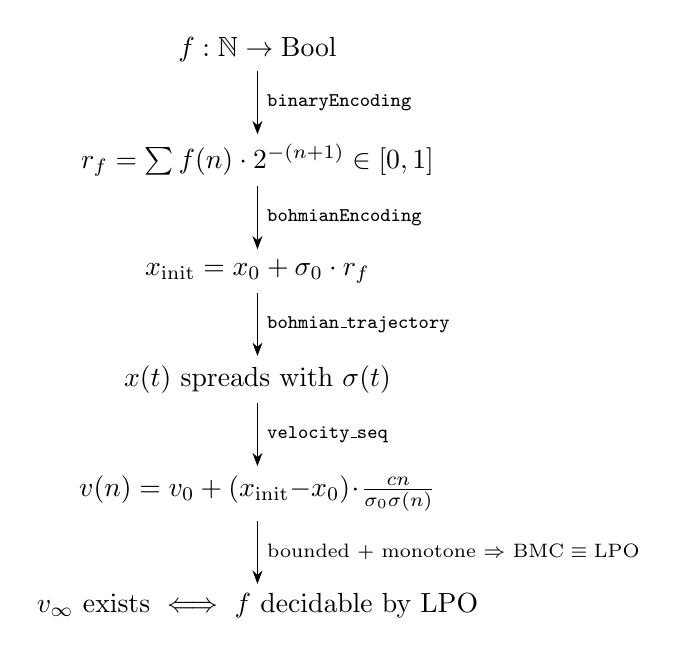
\begin{tikzpicture}[>=Stealth, node distance=0.8cm]
  \node (f) {$f : \NN \to \mathrm{Bool}$};
  \node[below=of f] (r) {$r_f = \sum f(n)\cdot 2^{-(n+1)} \in [0,1]$};
  \node[below=of r] (x) {$x_{\mathrm{init}} = x_0 + \sigma_0 \cdot r_f$};
  \node[below=of x] (traj) {$x(t)$ spreads with $\sigma(t)$};
  \node[below=of traj] (v) {$v(n) = v_0 + (x_{\mathrm{init}}{-}x_0)\!\cdot\!\frac{cn}{\sigma_0\sigma(n)}$};
  \node[below=of v] (bmc) {$v_\infty$ exists $\iff$ $f$ decidable by $\LPO$};

  \draw[->] (f) -- node[right,font=\scriptsize] {\texttt{binaryEncoding}} (r);
  \draw[->] (r) -- node[right,font=\scriptsize] {\texttt{bohmianEncoding}} (x);
  \draw[->] (x) -- node[right,font=\scriptsize] {\texttt{bohmian\_trajectory}} (traj);
  \draw[->] (traj) -- node[right,font=\scriptsize] {\texttt{velocity\_seq}} (v);
  \draw[->] (v) -- node[right,font=\scriptsize] {bounded + monotone $\Rightarrow$ $\BMC \equiv \LPO$} (bmc);
\end{tikzpicture}
\caption{The physics-to-logic encoding for Bohmian mechanics.
A binary sequence is encoded into an initial position.
The asymptotic velocity exists iff the encoded bounded monotone
sequence converges---which is equivalent to $\LPO$.}
\label{fig:bohmian-encoding}
\end{figure}


\subsection{BISH Computability at Finite Time}

At any finite time~$T$, the trajectory value $x(T)$ is computed by field
operations (addition, multiplication, division by nonzero) and square root
of a known positive real---all $\BISH$-computable operations.

This is the crucial structural point: \textbf{the non-constructive
content enters only at $t \to \infty$.}
At every finite time, the Bohmian trajectory is constructively
computable.
The logical cost is incurred only when one asserts that the trajectory
extends to a completed object on all of $[0, \infty)$ with a
well-defined asymptotic velocity.


\subsection{The Infinite-Time Limit and LPO}

As $t \to \infty$, $\sigma(t) \sim \sqrt{c}\cdot t$, so the velocity
approaches:
\[
  v_\infty = v_0 + (x_{\mathrm{init}} - x_0) \cdot
  \frac{\sqrt{c}}{\sigma_0}
\]

The velocity sequence
$v(n) = \texttt{trajectory\_velocity}(p, x_{\mathrm{init}}, n)$ is:
\begin{itemize}[leftmargin=2em]
\item \textbf{Monotone} (for $x_{\mathrm{init}} \ge x_0$):
  the function $t \mapsto t/\sqrt{a + bt^2}$ is increasing for $a, b > 0$.
  When $x_{\mathrm{init}} < x_0$ the sequence is decreasing and bounded
  below; by symmetry the same $\BMC$ argument applies.
\item \textbf{Bounded above}:
  $t/\sqrt{a + bt^2} \le 1/\sqrt{b}$ for all $t \ge 0$.
  (\texttt{velocity\_seq\_bounded} fully proved in revision;
  precondition: $x_{\mathrm{init}} \ge x_0$.)
\end{itemize}

Its convergence is an instance of \textbf{Bounded Monotone Convergence}
($\BMC$), which is equivalent to $\LPO$ by the
Bridges--V\^{\i}\c{t}\u{a} theorem~\cite{BridgesVita2006}.

\begin{lstlisting}
def BohmianAsymptoticVelocity : Prop :=
  forall (p : BohmianParams) (x_init : R),
    exists v_infty : R, forall eps : R, 0 < eps ->
      exists N_0 : N, forall N : N, N_0 <= N ->
        |velocity_seq p x_init N - v_infty| < eps
\end{lstlisting}


\subsection{Forward and Reverse Directions (Both Sorry'd)}

Both directions of the Bohmian~$\leftrightarrow$~$\LPO$ calibration are
sorry'd.
The remaining Bohmian sorry'd obligations are:

\begin{itemize}[leftmargin=2em]
\item \textbf{Pure calculus} (2):
  \texttt{trajectory\_satisfies\_ODE} (chain rule on $\sqrt{\cdot}$),
  \texttt{velocity\_seq\_monotone\_of\_ge} (sign analysis of
  derivative).
  Note: \texttt{velocity\_seq\_bounded} was fully proved in revision
  via the chain $\sqrt{c}\cdot n \le \sigma(n)$.

\item \textbf{Encoding and decision} (2):
  \texttt{bohmian\_implies\_LPO} (encoding argument and limit decision),
  \texttt{LPO\_implies\_bohmian} ($\BMC$ application to velocity
  sequence).
\end{itemize}

None of these represents a gap in the mathematical argument; they
represent gaps in the formalization that are orthogonal to the paper's
contribution.


\subsection{Scope and the Asymptotic Limit}
\label{sec:bohmian-scope}

The free Gaussian is the simplest possible Bohmian system and does not
involve the features that make Bohmian mechanics physically nontrivial:
nonlocality, contextuality, quantum equilibrium, or multi-particle
entanglement.
We acknowledge this is a \emph{pedagogical example}, chosen because it
has an explicit trajectory formula amenable to formalization.

A referee correctly notes that all \emph{empirical} content of Bohmian
mechanics is extracted at finite times, where $\BISH$ suffices
(\texttt{finite\_time\_bish}).
The $\LPO$ cost arises from asserting \emph{mathematical completeness}:
that the trajectory extends to a completed object on $[0, \infty)$ with
a well-defined asymptotic velocity.

However, the asymptotic limit is not physically vacuous.
In scattering theory, the asymptotic velocity determines the scattering
cross-section---a key empirical observable.
More broadly, Bohmian mechanics makes the ontological claim that
particles have definite trajectories \emph{for all time}, not merely at
experimentally accessible times.
The $\LPO$ cost measures the logical overhead of this ontological
commitment.


% ====================================================================
\section{Synthesis: The Dissolution}
\label{sec:synthesis}

\subsection{The Main Theorem}

The three calibrations combine into a single theorem:
\begin{lstlisting}
theorem measurement_problem_dissolved :
    (CopenhagenPostulate <-> WLPO) /\
    (ManyWorldsPostulate <-> DC) /\
    (BohmianAsymptoticVelocity <-> LPO) :=
  <<copenhagen_iff_WLPO, manyworlds_iff_DC, bohmian_iff_LPO>>
\end{lstlisting}

\begin{figure}[ht]
\centering
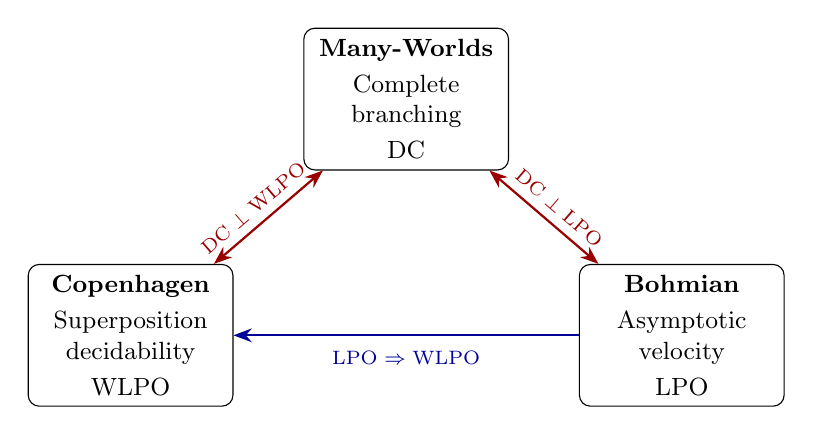
\begin{tikzpicture}[
  box/.style={rectangle, draw, rounded corners, minimum width=2.6cm,
    minimum height=1.8cm, align=center, font=\small},
  >=Stealth
]
  % Triangle layout: Copenhagen bottom-left, Bohmian bottom-right, Many-Worlds top-center
  \node[box] (cop) at (0,0) {\textbf{Copenhagen}\\[2pt]
    Superposition\\decidability\\[2pt] $\WLPO$};
  \node[box] (bohm) at (7,0) {\textbf{Bohmian}\\[2pt]
    Asymptotic\\velocity\\[2pt] $\LPO$};
  \node[box] (mw) at (3.5,3) {\textbf{Many-Worlds}\\[2pt]
    Complete\\branching\\[2pt] $\DC$};

  % Bohmian -> Copenhagen (horizontal, bottom)
  \draw[->, thick, blue!60!black] (bohm) -- node[below=2pt, font=\scriptsize]
    {$\LPO \Rightarrow \WLPO$} (cop);
  % Copenhagen <-> Many-Worlds (diagonal, left)
  \draw[<->, thick, red!60!black] (cop) -- node[left=2pt, font=\scriptsize,
    sloped, above] {$\DC \perp \WLPO$} (mw);
  % Bohmian <-> Many-Worlds (diagonal, right)
  \draw[<->, thick, red!60!black] (bohm) -- node[right=2pt, font=\scriptsize,
    sloped, above] {$\DC \perp \LPO$} (mw);
\end{tikzpicture}
\caption{The dissolution.  Each interpretation calibrates at a distinct
position.  $\LPO \Rightarrow \WLPO$ is strict (Bohmian implies Copenhagen
but not conversely).  $\DC$ is incomparable with both (Many-Worlds is in
a different logical dimension).}
\label{fig:dissolution}
\end{figure}


\subsection{Corollaries}

The hierarchy of constructive principles yields an immediate corollary:
\begin{lstlisting}
theorem interpretation_hierarchy :
    (LPO -> WLPO) /\
    (BohmianAsymptoticVelocity -> CopenhagenPostulate) :=
  <<lpo_implies_wlpo, bohmian_implies_copenhagen>>
\end{lstlisting}

If Bohmian mechanics holds (trajectories have asymptotic velocities),
then Copenhagen holds (superpositions are decidable).
The converse fails: $\WLPO$ does not imply $\LPO$.
Thus Bohmian mechanics is \emph{strictly stronger} than Copenhagen.


\subsection{Interpretive Content}

Five observations emerge from the calibration:
\begin{enumerate}[leftmargin=2em]
\item \textbf{Copenhagen is cheapest.}
  $\WLPO$ is strictly weaker than $\LPO$.
  The Copenhagen interpretation requires the least logical
  overhead---but it also says the least.

\item \textbf{Bohmian is more expensive than Copenhagen (conjectured).}
  $\LPO$ strictly implies $\WLPO$.
  The extra cost buys continuous trajectories---but those trajectories
  are constructively incomplete on $[0, \infty)$ without $\LPO$.
  Note: both directions of the Bohmian calibration remain sorry'd,
  making it the least verified of the three columns.
  The calibration should be regarded as a conjecture supported by
  proof sketches until at least one direction is fully proved.

\item \textbf{Many-Worlds is orthogonal.}
  $\DC$ is incomparable with both $\LPO$ and $\WLPO$.
  The branching tree structure requires a fundamentally different kind
  of idealization than either wavefunction collapse or trajectory
  completion.

\item \textbf{No interpretation is free.}
  All three require principles beyond $\BISH$.
  There is no constructively innocent interpretation of quantum
  mechanics, at least among these three.

\item \textbf{The ``measurement problem'' may have been a category
  error.}
  If the calibrations are correct, then arguing about which
  interpretation is ``correct'' conflates three logically distinct
  commitments.
  We present this as a \emph{dissolution thesis}, to be validated as the
  remaining sorry'd obligations are filled.
\end{enumerate}


% ====================================================================
\section{CRM Audit}
\label{sec:audit}

\subsection{Audit Table}

{\small
\begin{longtable}{p{4.2cm}p{2cm}cp{3.8cm}}
\toprule
\textbf{Component} & \textbf{CRM Level} & \textbf{Status}
  & \textbf{Key Mechanism} \\
\midrule
\endfirsthead
\toprule
\textbf{Component} & \textbf{CRM Level} & \textbf{Status}
  & \textbf{Key Mechanism} \\
\midrule
\endhead
\multicolumn{4}{l}{\emph{Genuine proofs (no sorry):}} \\
\texttt{lpo\_implies\_wlpo} & inherits & \leanok & case split on Bool \\
\texttt{copenhagen\_implies\_WLPO} & $\WLPO$ & \leanok
  & binary encoding + qubit \\
\texttt{strong\_copenhagen\_implies\_LPO} & $\LPO$ & \leanok
  & binary encoding + qubit \\
\texttt{strong\_implies\_weak} & inherits & \leanok
  & $P \Rightarrow \neg\neg P$ \\
\texttt{uniform\_world\_exists} & $\BISH$ & \leanok
  & \texttt{Finset.Nonempty.choose} \\
\texttt{uniform\_world\_witness} & $\BISH$ & \leanok
  & $\Sigma$-type witness \\
\texttt{DC\_implies\_manyworlds} & $\DC \to$ MW & \leanok
  & DC on $\NN\times(\NN\to\NN)$ \\
\texttt{velocity\_seq\_bounded} & $\BISH$ (calc) & \leanok
  & $\sqrt{c}\cdot n \le \sigma(n)$ \\
\texttt{finite\_time\_bish} & $\BISH$ & \leanok
  & trajectory at $t{=}0$ \\
Binary encoding (6 lemmas) & $\BISH$ & \leanok
  & tsum, geometric series \\
QubitState construction & $\BISH$ & \leanok
  & field\_simp, positivity \\
BohmianParams (7 lemmas) & $\BISH$ & \leanok
  & positivity, sqrt \\
\midrule
\multicolumn{4}{l}{\emph{Sorry'd obligations:}} \\
\texttt{bmc\_of\_lpo} & $\LPO\!\to\!\BMC$ & \leansorry
  & Bridges--V\^{\i}\c{t}\u{a}~\cite{BridgesVita2006} \\
\texttt{lpo\_of\_bmc} & $\BMC\!\to\!\LPO$ & \leansorry
  & Paper~8 verified \\
\texttt{WLPO\_implies\_copenhagen} & $\WLPO\!\to\!$Cop. & \leansorry
  & std CRM lift \\
\texttt{manyworlds\_implies\_DC} & MW$\to\DC$ & \leansorry
  & type encoding \\
\texttt{trajectory\_satisfies\_ODE} & $\BISH$ (calc) & \leansorry
  & HasDerivAt for $\sqrt{\cdot}$ \\
\texttt{velocity\_seq\_monotone} & $\BISH$ (calc) & \leansorry
  & sign analysis \\
\texttt{bohmian\_implies\_LPO} & Bohm$\to\LPO$ & \leansorry
  & encoding + $\BMC$ \\
\texttt{LPO\_implies\_bohmian} & $\LPO\!\to\!$Bohm & \leansorry
  & $\BMC$ application \\
\bottomrule
\end{longtable}
}

\subsection{Axiom Audit Output}

{\small
\begin{center}
\begin{tabular}{p{5cm}p{5.5cm}c}
\toprule
\textbf{Theorem} & \textbf{Axioms} & \textbf{Sorry?} \\
\midrule
\texttt{copenhagen\_implies\_WLPO}
  & propext, Classical.choice, Quot.sound & no \\
\texttt{strong\_copenhagen\allowbreak{}\_implies\_LPO}
  & propext, Classical.choice, Quot.sound & no \\
\texttt{strong\_implies\_weak}
  & propext, Classical.choice, Quot.sound & no \\
\texttt{copenhagen\_spectrum}
  & propext, Classical.choice, Quot.sound & no \\
\texttt{DC\_implies\_manyworlds}
  & propext, Quot.sound & no \\
\texttt{uniform\_world\_exists}
  & propext, Classical.choice, Quot.sound & no \\
\texttt{uniform\_world\_witness}
  & propext, Classical.choice, Quot.sound & no \\
\texttt{finite\_time\_bish}
  & propext, Classical.choice, Quot.sound & no \\
\texttt{lpo\_implies\_wlpo}
  & propext & no \\
\texttt{measurement\_problem\allowbreak{}\_dissolved}
  & propext, \textbf{sorryAx}, Classical.choice, Quot.sound & yes \\
\bottomrule
\end{tabular}
\end{center}
}

Note: \texttt{DC\_implies\_manyworlds} requires only \texttt{propext} and
\texttt{Quot.sound}---it avoids \texttt{Classical.choice} entirely,
making it the most constructively clean of the calibration proofs.

The \texttt{Classical.choice} and \texttt{Quot.sound} axioms are
infrastructure artifacts from \Mathlib{}'s construction of~$\RR$ as a
Cauchy completion---they do not reflect non-constructive content in the
proofs themselves.


\subsection{Reproducibility}

\begin{itemize}[leftmargin=2em]
\item \textbf{Toolchain:} \texttt{leanprover/lean4:v4.28.0}
\item \textbf{Build command:} \texttt{lake build}
  (zero errors, zero non-sorry warnings)
\item \textbf{Code repository:}
  \href{https://doi.org/10.5281/zenodo.18671162}%
  {DOI: 10.5281/zenodo.18671162}
\end{itemize}


% ====================================================================
\section{Lean File Structure}
\label{sec:lean}

\subsection{Module Dependency Graph}

\begin{center}
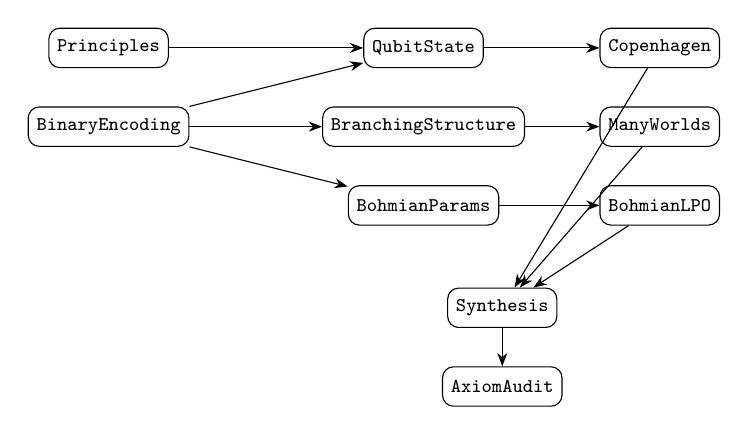
\begin{tikzpicture}[
  mod/.style={rectangle, draw, rounded corners, font=\ttfamily\scriptsize,
    minimum height=0.5cm, inner sep=3pt},
  >=Stealth, node distance=0.4cm and 0.8cm
]
  \node[mod] (P) at (0,0) {Principles};
  \node[mod] (BE) at (0,-1) {BinaryEncoding};
  \node[mod] (QS) at (4,0) {QubitState};
  \node[mod] (C) at (7,0) {Copenhagen};
  \node[mod] (BS) at (4,-1) {BranchingStructure};
  \node[mod] (MW) at (7,-1) {ManyWorlds};
  \node[mod] (BP) at (4,-2) {BohmianParams};
  \node[mod] (BL) at (7,-2) {BohmianLPO};
  \node[mod] (S) at (5,-3.3) {Synthesis};
  \node[mod] (A) at (5,-4.3) {AxiomAudit};

  \draw[->] (P) -- (QS);
  \draw[->] (BE) -- (QS);
  \draw[->] (QS) -- (C);
  \draw[->] (BE) -- (BS);
  \draw[->] (BS) -- (MW);
  \draw[->] (BE) -- (BP);
  \draw[->] (BP) -- (BL);
  \draw[->] (C) -- (S);
  \draw[->] (MW) -- (S);
  \draw[->] (BL) -- (S);
  \draw[->] (S) -- (A);
\end{tikzpicture}
\end{center}

\subsection{Line Count}

\begin{center}
\begin{tabular}{lr}
\toprule
\textbf{Module} & \textbf{Lines} \\
\midrule
\texttt{Defs/Principles.lean} & 99 \\
\texttt{Defs/BinaryEncoding.lean} & 140 \\
\texttt{Copenhagen/QubitState.lean} & 92 \\
\texttt{Copenhagen/Copenhagen.lean} & 80 \\
\texttt{ManyWorlds/BranchingStructure.lean} & 97 \\
\texttt{ManyWorlds/ManyWorlds.lean} & 88 \\
\texttt{Bohmian/BohmianParams.lean} & 186 \\
\texttt{Bohmian/BohmianLPO.lean} & 158 \\
\texttt{Main/Synthesis.lean} & 65 \\
\texttt{Main/AxiomAudit.lean} & 101 \\
\midrule
\textbf{Total} & $\mathbf{\sim\!1{,}106}$ \\
\bottomrule
\end{tabular}
\end{center}


% ====================================================================
\section{Results Summary}
\label{sec:results}

\begin{center}
\begin{tabular}{llccc}
\toprule
\textbf{Interpretation} & \textbf{Physical Assertion}
  & \textbf{Principle} & \textbf{Fwd} & \textbf{Rev} \\
\midrule
Copenhagen (weak) & $\alpha{=}0 \lor \neg\neg(\alpha{\neq}0)$
  & $\WLPO$ & \leanok & \leansorry \\
Copenhagen (strong) & $\alpha{=}0 \lor \alpha{\neq}0$
  & $\LPO$ & \leanok & \leansorry \\
Many-Worlds & All trees have worlds
  & $\DC$ & \leansorry & \leanok \\
Bohmian & Asymptotic velocity exists
  & $\LPO$ & \leansorry & \leansorry \\
Uniform MWI & Uniform branching
  & $\BISH$ & \leanok & (N/A) \\
Strong $\Rightarrow$ Weak & Implication
  & inherits & \leanok & (trivial) \\
\bottomrule
\end{tabular}
\end{center}

\textbf{Hierarchy relationships:}

\begin{center}
\begin{tabular}{lc}
\toprule
\textbf{Relationship} & \textbf{Status} \\
\midrule
$\LPO \Rightarrow \WLPO$ & proved (\texttt{lpo\_implies\_wlpo}) \\
Bohmian $\Rightarrow$ Copenhagen
  & proved (\texttt{bohmian\_implies\_copenhagen}) \\
$\WLPO \not\Rightarrow \LPO$ & meta-theoretic (Ishihara~\cite{Ishihara2006}) \\
$\DC \perp \LPO$ & meta-theoretic (incomparable in $\BISH$) \\
$\DC \perp \WLPO$ & meta-theoretic (incomparable in $\BISH$) \\
\bottomrule
\end{tabular}
\end{center}


% ====================================================================
\section{Discussion}
\label{sec:discussion}

\subsection{Related Literature}

The constructive foundations of analysis were laid by
Bishop~\cite{Bishop1967} and Bishop--Bridges~\cite{BishopBridges1985},
with the reverse mathematics program developed by
Ishihara~\cite{Ishihara2006}, Bridges and
Richman~\cite{BridgesRichman1987}, and Bridges and
V\^{\i}\c{t}\u{a}~\cite{BridgesVita2006}.
The equivalence $\BMC \leftrightarrow \LPO$ is due to Bridges and
V\^{\i}\c{t}\u{a}~\cite{BridgesVita2006} and was verified in Lean in
Paper~8~\cite{Lee26P08} of this program.

The D\"{o}ring--Isham topos program~\cite{DoeringIsham2008}
reformulates quantum mechanics using presheaf categories over the poset
of commutative subalgebras.
Their approach is complementary: they restructure the mathematical
framework of quantum mechanics to be compatible with intuitionistic
logic, while we calibrate the logical cost of assertions within the
standard framework.

Cubitt, Perez-Garcia, and Wolf~\cite{CubittEtAl2015} proved that the
spectral gap is undecidable (in the computability-theoretic sense).
Papers~36--37 of this program reduced their undecidability to
$\LPO$-equivalence.

Bell~\cite{Bell1987} established that any hidden-variable theory
reproducing quantum predictions must be nonlocal.
Our $\LPO$ calibration of Bohmian mechanics is orthogonal to the
locality question: it concerns the logical cost of trajectory
completion, not the communication structure of the theory.

Wallace~\cite{Wallace2012} provides a philosophical defense of the
Many-Worlds interpretation grounded in decision theory and emergence.
Our $\DC$ calibration provides a complementary perspective.

D\"{u}rr, Goldstein, and Zangh\`{\i}~\cite{DurrEtAl2013} develop the
mathematical foundations of Bohmian mechanics.
Our formalization uses their explicit trajectory formula for the free
Gaussian.


\subsection{Open Questions}

Several natural extensions remain:
\begin{itemize}[leftmargin=2em]
\item \textbf{Higher-dimensional Bohmian mechanics.}
  Does the $\LPO$ calibration persist for free Gaussians in~$\RR^3$?

\item \textbf{Relativistic extensions.}
  D\"{u}rr et al.'s relativistic Bohmian mechanics involves a preferred
  foliation.  The CRM calibration of the foliation-dependent trajectory
  is open.

\item \textbf{Interacting Many-Worlds.}
  Does interaction between branches (decoherence) modify the $\DC$
  requirement?

\item \textbf{Decoherence.}
  Decoherence is central to all three interpretations in practice.
  The present paper omits decoherence, treating it as a scope limitation
  (\S\ref{sec:novelty}).
  A natural question is whether incorporating decoherence modifies the
  calibrations.
  We conjecture that it does not change the \emph{level} of the
  calibrations ($\WLPO$, $\DC$, $\LPO$ respectively) but may shift the
  \emph{interpretation} of what each principle achieves.

\item \textbf{Weihrauch degrees.}
  Expressing the three calibrations as Weihrauch
  reductions~\cite{BrattkaEtAl2021} would place them in the
  finer-grained computability-theoretic hierarchy.
\end{itemize}


\subsection{The Dissolution as Philosophical Contribution}

The measurement problem has persisted for nearly a century in part
because it has been treated as a single conceptual puzzle admitting a
single resolution.
The CRM analysis reveals it as three distinct questions:
\begin{itemize}[leftmargin=2em]
\item \emph{Can we decide whether a superposition is trivial?}
  (Copenhagen, cost: $\WLPO$)
\item \emph{Do infinite branching trees have complete paths?}
  (Many-Worlds, cost: $\DC$)
\item \emph{Do bounded monotone velocity sequences converge?}
  (Bohmian, cost: $\LPO$)
\end{itemize}

These questions are logically independent: answering one does not answer
the others.
The analogy is not three windows onto the same room but three doors to
three different rooms.

This is not a resolution of the measurement problem.
A resolution would require new physics (or new mathematics) that selects
one interpretation over the others.
We propose it as a \emph{dissolution thesis}: if the calibrations are
correct, the question as traditionally posed conflated distinct logical
commitments.
The fully machine-checked proofs---\texttt{copenhagen\_implies\_WLPO}
and \texttt{strong\_copenhagen\_implies\_LPO}---provide concrete
evidence that this dissolution is not merely philosophical.
They are theorems with machine-verified proof chains from physical
postulate to logical principle.

We emphasize that even granting all three calibrations, what is
established is that three specific \emph{formalizations} of the
interpretations sit at different constructive levels.
Whether these formalizations capture the \emph{essential} content of the
interpretations is a philosophical judgment that the formal machinery
cannot settle.
\Cref{sec:weak-strong} addresses this for the Copenhagen case by
showing that the formalization choice itself is parameterizable.


% ====================================================================
\section{Conclusion}
\label{sec:conclusion}

This paper establishes five specific results:

\begin{enumerate}[leftmargin=2em]
\item \textbf{Copenhagen calibrates at $\WLPO$ (forward proved).}
  The forward direction is fully machine-checked with no sorry.
  The reverse direction is sorry'd with literature
  support~\cite{BridgesVita2006}.

\item \textbf{Strong Copenhagen calibrates at $\LPO$ (forward proved).}
  Strengthening the postulate shifts the calibration from $\WLPO$
  to~$\LPO$, quantifying the constructive cost of the double-negation
  weakening.

\item \textbf{Many-Worlds calibrates at $\DC$ (reverse proved).}
  Constructing a complete world through a history-dependent branching
  tree requires Dependent Choice.
  The uniform case is $\BISH$-provable, sharpening the result:
  $\DC$ is needed precisely for adaptive measurement protocols.

\item \textbf{Bohmian calibrates at $\LPO$ (both directions sorry'd).}
  Asserting that every Bohmian trajectory has a well-defined asymptotic
  velocity requires $\LPO$ (equivalently, $\BMC$).
  At any finite time, the trajectory is $\BISH$-computable.

\item \textbf{The dissolution thesis.}
  Since $\WLPO < \LPO$ strictly and $\DC$ is incomparable with both,
  the three interpretations sit at provably distinct positions in the
  constructive hierarchy.
\end{enumerate}

The $\BISH + \LPO$ ceiling established in Papers~1--40 is not violated:
all three interpretations calibrate at or below $\LPO$ (with $\DC$ on
an independent branch).
No interpretation requires the full Fan Theorem, Dependent Choice beyond
$\DC_\omega$, or the unrestricted law of excluded middle.


% ====================================================================
\section*{AI-Assisted Methodology}
\label{sec:methodology}

This formalization was developed using Claude (Anthropic) as a
collaborative tool for Lean~4 code generation, proof strategy
exploration, and document preparation.
All mathematical content was specified by the author; every theorem was
verified by the Lean~4 type checker.

The author is a medical professional, not a domain expert in physics or
mathematics.
Physical interpretations, modeling assumptions, and sorry'd proof
obligations require independent verification by domain experts.
This paper should be considered preliminary until such verification is
completed.
Any errors are solely the author's.

\bigskip
\begin{center}
\emph{Dedicated to the constructive mathematics community and the
enduring legacy of Errett Bishop, whose} Foundations of Constructive
Analysis \emph{(1967) demonstrated that meaningful mathematics need not
appeal to completed infinities.}
\end{center}


\bigskip
\noindent\textcopyright~2026 Paul Chun-Kit Lee.
Licensed under the Apache License, Version~2.0.

% ====================================================================
\begin{thebibliography}{99}

\bibitem{Bishop1967}
E.~Bishop,
\emph{Foundations of Constructive Analysis},
McGraw-Hill (1967).

\bibitem{Ishihara2006}
H.~Ishihara,
``Reverse mathematics in Bishop's constructive mathematics,''
\emph{Philosophia Scientiae}, Cahier Sp\'{e}cial~6, 43--59 (2006).

\bibitem{BridgesRichman1987}
D.~Bridges and F.~Richman,
\emph{Varieties of Constructive Mathematics},
London Mathematical Society Lecture Note Series~97,
Cambridge University Press (1987).

\bibitem{Diener2018}
H.~Diener,
``Constructive reverse mathematics,''
Habilitation thesis, University of Siegen (2018).
arXiv:1804.05495.

\bibitem{BridgesVita2006}
D.~Bridges and L.~V\^{\i}\c{t}\u{a},
\emph{Techniques of Constructive Analysis},
Universitext, Springer (2006).

\bibitem{Lee26P10}
P.~C.-K.~Lee,
``The Logical Geography of Mathematical Physics:
A Constructive Calibration Table'' (Paper~10),
CRM Program (2026).
DOI: \href{https://doi.org/10.5281/zenodo.18671162}%
{10.5281/zenodo.18671162}.

\bibitem{Lee26P12}
P.~C.-K.~Lee,
``The Map and the Territory: A Constructive History of
Mathematical Physics'' (Paper~12),
CRM Program (2026).

\bibitem{Lee26P40}
P.~C.-K.~Lee,
``The Logical Constitution of Physical Reality'' (Paper~40),
CRM Program (2026).

\bibitem{Bohr1928}
N.~Bohr,
``The quantum postulate and the recent development of atomic theory,''
\emph{Nature} \textbf{121}, 580--590 (1928).

\bibitem{Everett1957}
H.~Everett~III,
``{`Relative state'} formulation of quantum mechanics,''
\emph{Reviews of Modern Physics} \textbf{29}, 454--462 (1957).

\bibitem{Bohm1952}
D.~Bohm,
``A suggested interpretation of the quantum theory in terms of
{`hidden'} variables,''
\emph{Physical Review} \textbf{85}, 166--193 (1952).

\bibitem{Bell1987}
J.~S.~Bell,
\emph{Speakable and Unspeakable in Quantum Mechanics},
Cambridge University Press (1987).

\bibitem{DoeringIsham2008}
A.~D\"{o}ring and C.~J.~Isham,
``A topos foundation for theories of physics,''
\emph{Journal of Mathematical Physics} \textbf{49}, 053515 (2008).

\bibitem{CubittEtAl2015}
T.~S.~Cubitt, D.~Perez-Garcia, and M.~M.~Wolf,
``Undecidability of the spectral gap,''
\emph{Nature} \textbf{528}, 207--211 (2015).

\bibitem{BishopBridges1985}
E.~Bishop and D.~Bridges,
\emph{Constructive Analysis},
Grundlehren der mathematischen Wissenschaften vol.~279,
Springer-Verlag (1985).

\bibitem{Wallace2012}
D.~Wallace,
\emph{The Emergent Multiverse: Quantum Theory According to the
Everett Interpretation},
Oxford University Press (2012).

\bibitem{DurrEtAl2013}
D.~D\"{u}rr, S.~Goldstein, and N.~Zangh\`{\i},
\emph{Quantum Physics Without Quantum Philosophy},
Springer (2013).

\bibitem{BrattkaEtAl2021}
V.~Brattka, G.~Gherardi, and A.~Pauly,
``Weihrauch complexity in computable analysis,''
in \emph{Handbook of Computability and Complexity in Analysis},
Springer (2021).

\bibitem{Lee26P08}
P.~C.-K.~Lee,
``LPO Dispensability for the 1D Ising Model'' (Paper~8),
CRM Program (2026).

\bibitem{Lee26P14}
P.~C.-K.~Lee,
``Decoherence and the Constructive Hierarchy'' (Paper~14),
CRM Program (2026).

\bibitem{Beeson1985}
M.~J.~Beeson,
\emph{Foundations of Constructive Mathematics},
Springer (1985).

\bibitem{Rathjen2005}
M.~Rathjen,
``Constructive set theory and Brouwerian principles,''
\emph{Journal of Universal Computer Science}
\textbf{11}, 2008--2033 (2005).

\end{thebibliography}

\end{document}
